\section{\label{sec:intro}Introduction}


In recent years, there has been an increasing interest in tasks that require generating natural language, including
  abstractive summarization~\citep{nallapati2016abstractive},
  open-response question answering~\citep{nguyen2016ms,kovcisky2017narrativeqa}, 
  image captioning~\citep{lin2014microsoft},
  and open-domain dialogue~\citep{lowe2017ubuntu}.
Unfortunately, the evaluation of these systems remains a thorny issue because of the diversity of possible correct responses.
As the gold standard of performing human evaluation is often too expensive,
there has been a large effort developing
automatic metrics such as BLEU~\citep{papineni02bleu}, ROUGE~\citep{lin2004rouge}, METEOR~\citep{lavie2009meteor,denkowski2014meteor} and CiDER~\citep{vedantam2015cider}.
However, these have shown to be biased, correlating poorly with human metrics across different datasets and systems~\citep{liu2016evaluate,novikova2017why}.

\begin{figure*}[ht]
  \begin{subfigure}{0.49\textwidth}
    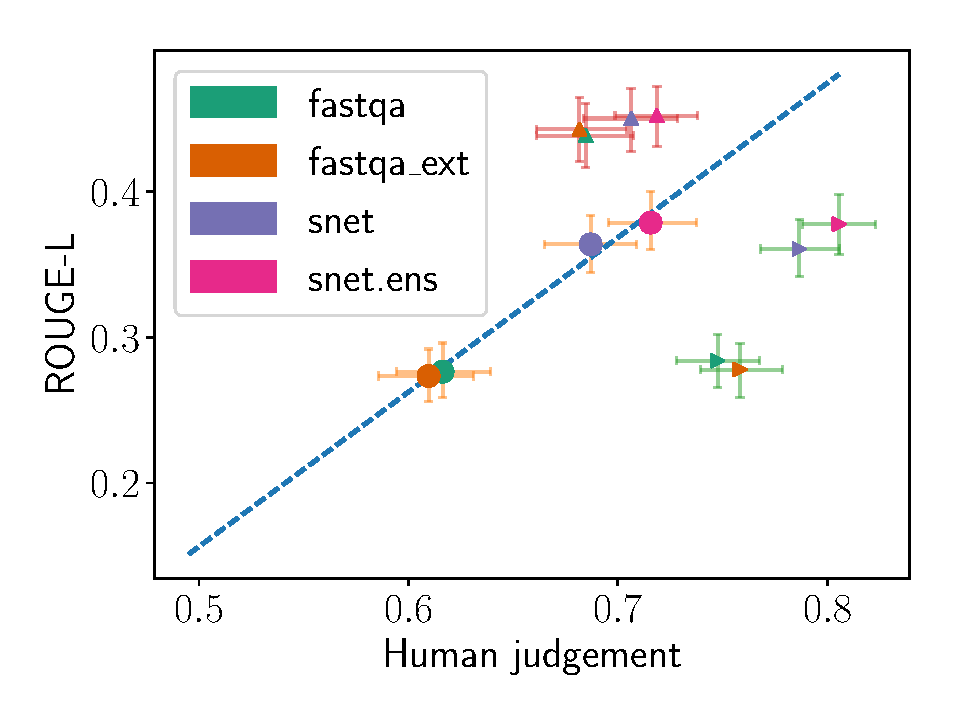
\includegraphics[width=\textwidth]{figures/msmarco_bias}
    \caption{\label{fig:bias-msmarco-system} System-level correlation on the MS MARCO task}
  \end{subfigure}
  \hfill
  \begin{subfigure}{0.49\textwidth}
    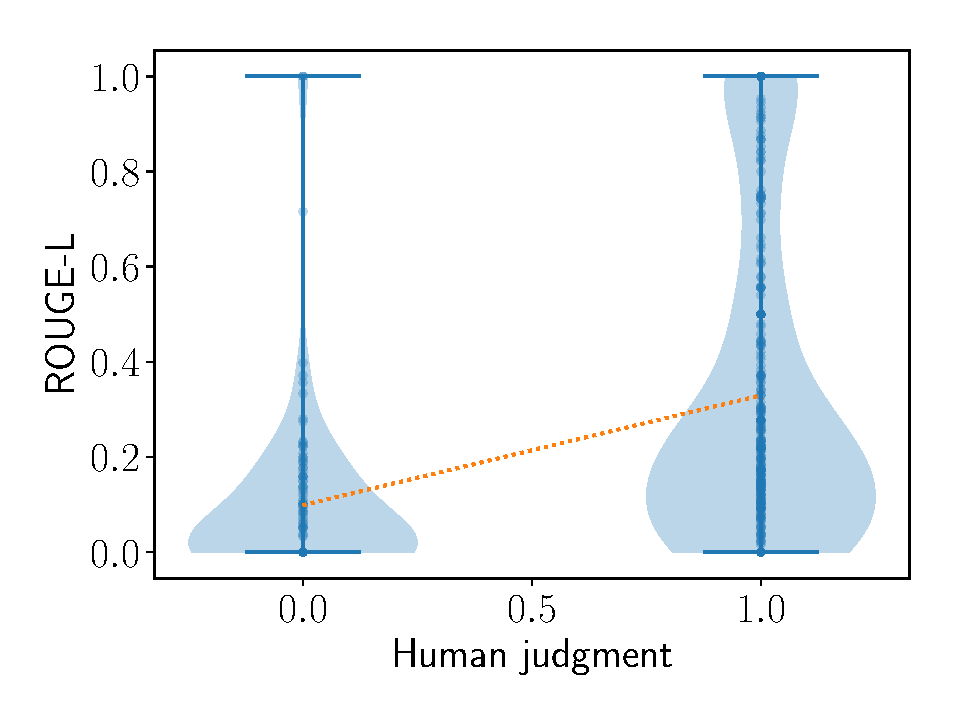
\includegraphics[width=\textwidth]{figures/msmarco_instance_correlation}
    \caption{\label{fig:bias-msmarco-instance} Instance-level correlation for the \texttt{fastqa} system}
  \end{subfigure}
  \caption{\label{fig:bias-msmarco}
  (a) At a system-level, automatic metrics (ROUGE-L) and human judgment correlate well, but (b) the instance-level correlation plot
  (where each point is a system prediction) shows that the instance-level correlation is quite low ($\rho = 0.31$).
  As a consequence, if we try to locally improve systems to produce better answers ($\triangleright$ in (a)),
  they do not significantly improve ROUGE scores and vice versa ($\vartriangle$).
  }
\end{figure*}


Can we combine automatic metrics and human evaluation to obtain
an \emph{unbiased} estimate at \emph{lower cost} than human evaluation alone?
In this paper,
we propose a simple estimator based on control variates~\citep{ripley2009stochastic},
where we average differences between human judgments and automatic metrics
rather than averaging the human judgments alone.
Provided the two are correlated,
our estimator will have lower variance and thus reduce cost.

We prove that our estimator is \emph{optimal} in the sense
that no unbiased estimator using the same automatic metric can have lower variance.
We also analyze its data efficiency (equivalently, cost savings)---the factor reduction in number of human judgments needed to obtain the same accuracy versus naive human evaluation---and show that it depends solely on
two factors:
  (a) the annotator variance (which is a function of the human evaluation prompt) and
  (b) the correlation between human judgments and the automatic metric.
This factorization allows us to calculate typical and best-case data efficiencies and accordingly refine the evaluation prompt or automatic metric.

Finally, we evaluate our estimator on state-of-the-art systems from two tasks, summarization on the CNN/Daily Mail dataset~\cite{hermann2015read,nallapati2016abstractive}
and open-response question answering on the MS MARCOv1.0 dataset~\citep{nguyen2016ms}.
To study our estimators offline,
we preemptively collected 10,000 human judgments which cover several tasks and systems.\footnote{%
An anonymized version of this data and the annotation interfaces used can be found at \url{https://bit.ly/price-of-debiasing}.}
As predicted by the theory, we find that the data efficiency depends not only on the correlation between the human and automatic metrics,
but also on the evaluation prompt.
If the automatic metric had perfect correlation, our data efficiency would be around 3, while
  if we had noiseless human judgments, our data efficiency would be about 1.5.
In reality, the reduction in cost we obtained was only about 10\%,
suggesting that improvements in both automatic metric and evaluation prompt are needed.
As one case study in improving the latter, we show that, when compared to a Likert survey, measuring the amount of post-editing needed to fix a generated sentence
reduced the annotator variance by three-fold.



